\newpage
\section{Topologisches Konzept}
Die topologische Überlegung spielt in der Umsetzung eine zentralle Rolle. Die zentrale Aufgabe des Projektes ist es Drohnen zu verwalten, welche sich in einem geografischen Gebiet bewegen. Dieses Gebiet kann Hindernisse, Gebäude oder Bäume beinhalten, welche möglichst sicher umflogen werden müssen. Da die Drohnen meistens über keine Kollisionserkennung verfügen, ist es umso wichtiger, dass viele Gefahren bereits in der Planung der Mission ausgeschlossen werden können. Statische Objekte mit unterschiedlicher Höhe können einfach umflogen oder überflogen werden, sofern die Drohne 'weiss' wie diese flugtechnisch zu vermeiden sind. \\
\begin{figure}[h]
	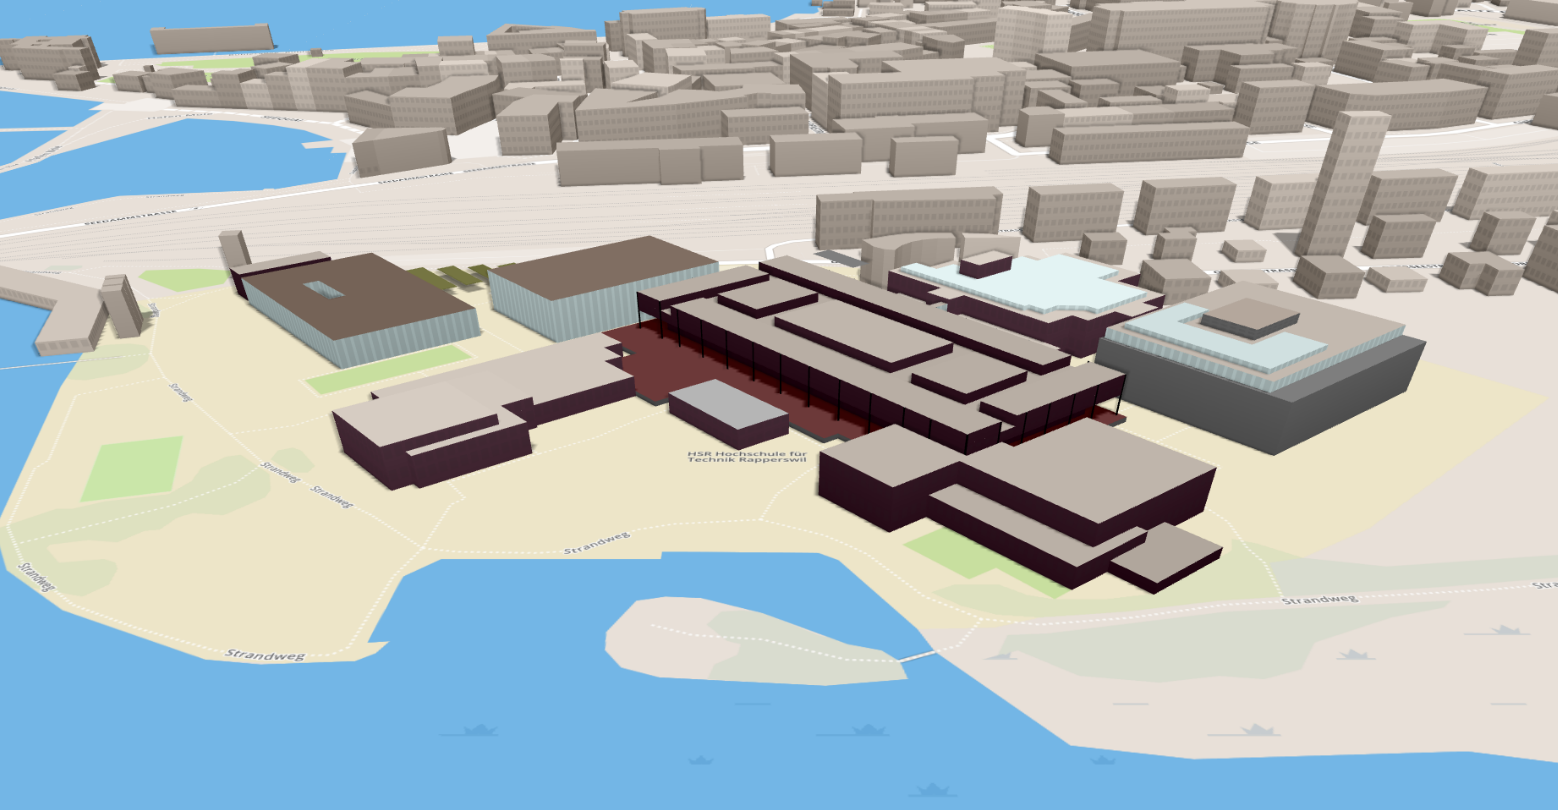
\includegraphics[width=1.0\textwidth]{images/routing/topology_example.png}
	\caption{Topologische Ansicht des Campus HSR}
	\label{fig:campus-hsr}
\end{figure}
\\
Am Beispiel der HSR ist unschwer zu erkennen, wie Gebäude in der Landschaft unteschiedliche Höhen haben. Diese Höhenunterschiede sollte wenn möglich gut in einem Model abgebildet werden können. \\
Aus diesen Überlegungen entstand das Zonen Model.
\subsection{Das Zonen Model}
Betrachten wir nun ein einfaches Projekt am Campus der HSR, so könnte dies wie folgt aussehen. \\
\begin{figure}[h]
	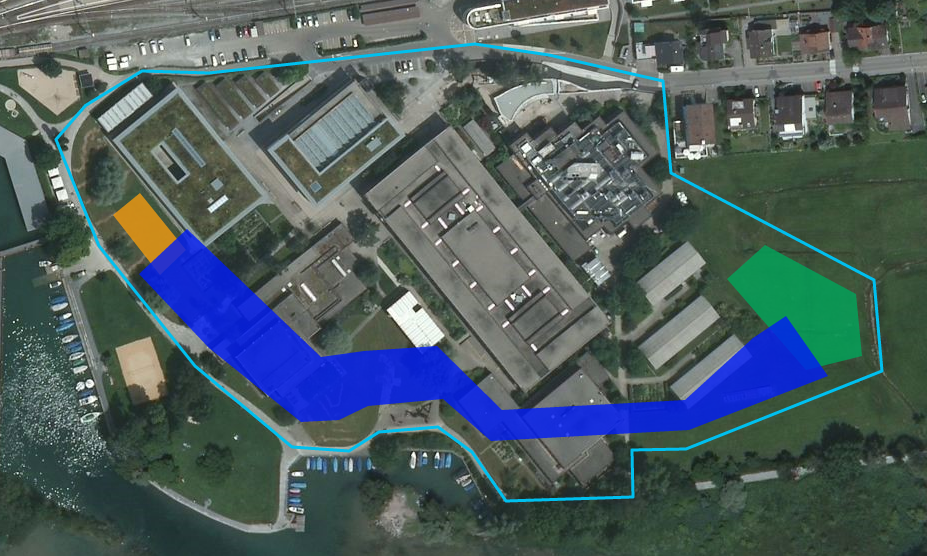
\includegraphics[width=1.0\textwidth]{images/routing/simpleProject_example.png}
	\caption{Einfaches Demo Projekt an der HSR}
	\label{fig:demo-project}
\end{figure}
Jedes Polygon bildet eine Zone ab. Diese Zonen können unterschiedliche Höhen aber auch Eigenschaften aufweisen. Die Höhe gewährleistet die minimale Flughöhe in einer Zone. Weiter unterscheiden wir 4 Zonentypen um die verschiedenen Operationen zu ermöglichen.
\begin{itemize}
	\item{\textbf{OrderZone:} Bereich in welchem Produkte im CustomerApp für dieses Projekt bestellt werden können.  (\textit{hell blauer Rahmen})}
	\item{\textbf{LoadingZone:} Zone die gebraucht wird um die Drohne zu beladen. (\textit{orange})}
	\item{\textbf{DeliveryZone:} Diese Zone definiert das Gebiet über welchem das Produkt abgeworfen werden kann. (\textit{grün})}
	\item{\textbf{FlightZone:} Die Flugzone verbindet die Ladezone mit der Abwurfzone. Weiter garantiert sie, dass die angegebene Flughöhe gewährleistet wird. (\textit{blau})}
\end{itemize}
\subsection{Routing-Algorithmus}
%Todo: Read that shit again!
Das Zonenmodel bringt lässt es einfach zu, dass Flugkoridore sehr intuitiv gebildet werden können. Leider eignen sich diese Polygone weniger gut für eine Navigation oder eine Routenberechnung. Die Routenberechnung im klassischen Sinne entsteht auf einem Graph. Anhand des Graphs wird mit Start und Endpunkt eine Lösung berechnet und diese stellt dann die Route dar. Da dieses Konzept naheliegend war, sollten die Polygone auf einen Graph reduziert werden.
\subsection{Reduktion vom Polygon zum Graph}
Für das Routing sind nur die drei Zonen, LoadingZone, DeliveryZone und FlightZone von entscheidender Bedeutung. Diese Zonen können von den Drohen überflogen werden, die OrderZone dient ausschliesslich um die richtigen Produkte im CustomerApp anzuzeigen. Um die Problemstellung etwas besser zu verstehen, haben wir mit einem Polygon angefangen um verschiedene Ansätze zu testen.
\subsubsection{Erste Konzept: Direkte Route}
Unser erstes Konzept umfasste den Ansatz den Start und den Endpunkt direkt zu verbinden, und dann grundsätzlich dem Rand nachzufligen. Diese Lösung an einem Beispiel sah folgendermassen aus.
\begin{figure}[h]
	\centering
	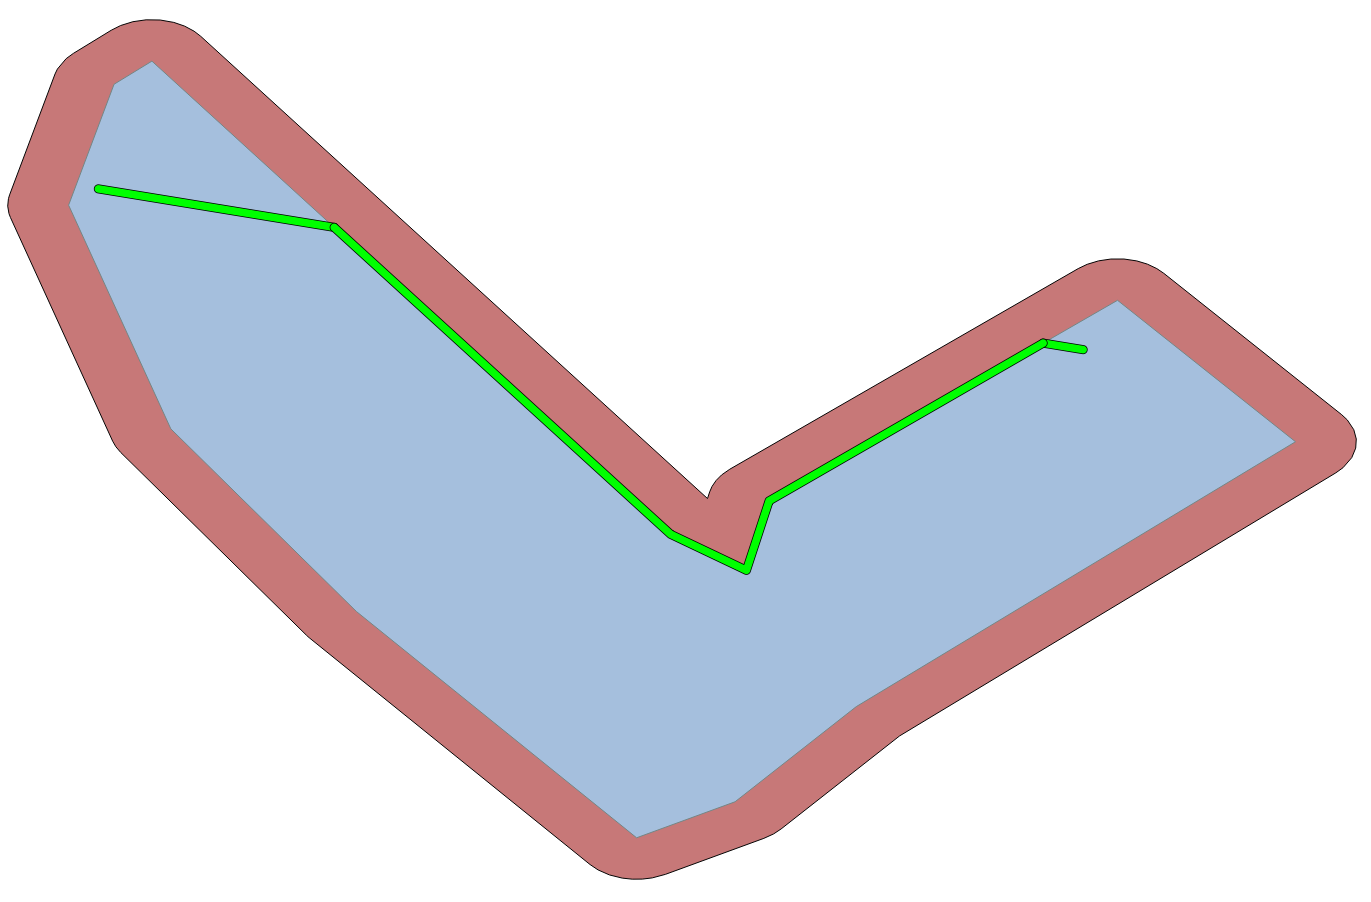
\includegraphics[width=0.8\textwidth]{images/routing/firstSolution.png}
	\caption{Erstes Konzept}
	\label{fig:first-concet-routing}
\end{figure}
Aus Sicherheitsgründen wurde ein zusätzlicher Rand (\textit{Rot}) berechnet. Das Ursprüngliche Polygon wurde um 5 Meter geschrumpft um nicht zu nah an den realen Rand des Polygons zu fliegen. Diese Massnahme wurde getroffen damit allfällige GPS Fehler keine Einfluss auf das Resulat haben. Die Drohen hat somit eine sicherheits marge für allfälige Flugfehler.
\\
So simpel dieses Konzept auch war, leider brachte es aber einige schwächen. Enge Korridore können so nicht gut durchflogen werden, und das verwenden des Randes stellt technisch keine esthetische Lösung dar.
\newpage
\subsubsection{Zweites Konzept: Visibility Graph}
Das nächste Konzept konzentrierte sich auf den 'Visibility Graphen'. 
\cite[p.1]{IEEEPaper} 
\blockquote{Using visibility graphs for determining the shortest path is very practical and intuitive. The visibility graph of a set of nonintersecting polygonal obstacles in the plane is an undirected graph whose vertices are the vertices of the obstacles and whose edges are pairs of vertices such that the open line segment between each two vertices does not intersect any of the obstacles.}
In unserem Fall haben wir den Gedanken umgedreht. Wir haben den Graphen in einem Polygon mit potentiellen Löchern berechnet. Diese Löcher stellen Enklaven für Bäume oder Gebäude dar. Das Konzept ist aber das gleiche, angewendet auf unser Beispiel Polygon ergibt sich folgende Abstraktion:
\begin{figure}[h]
	\centering
	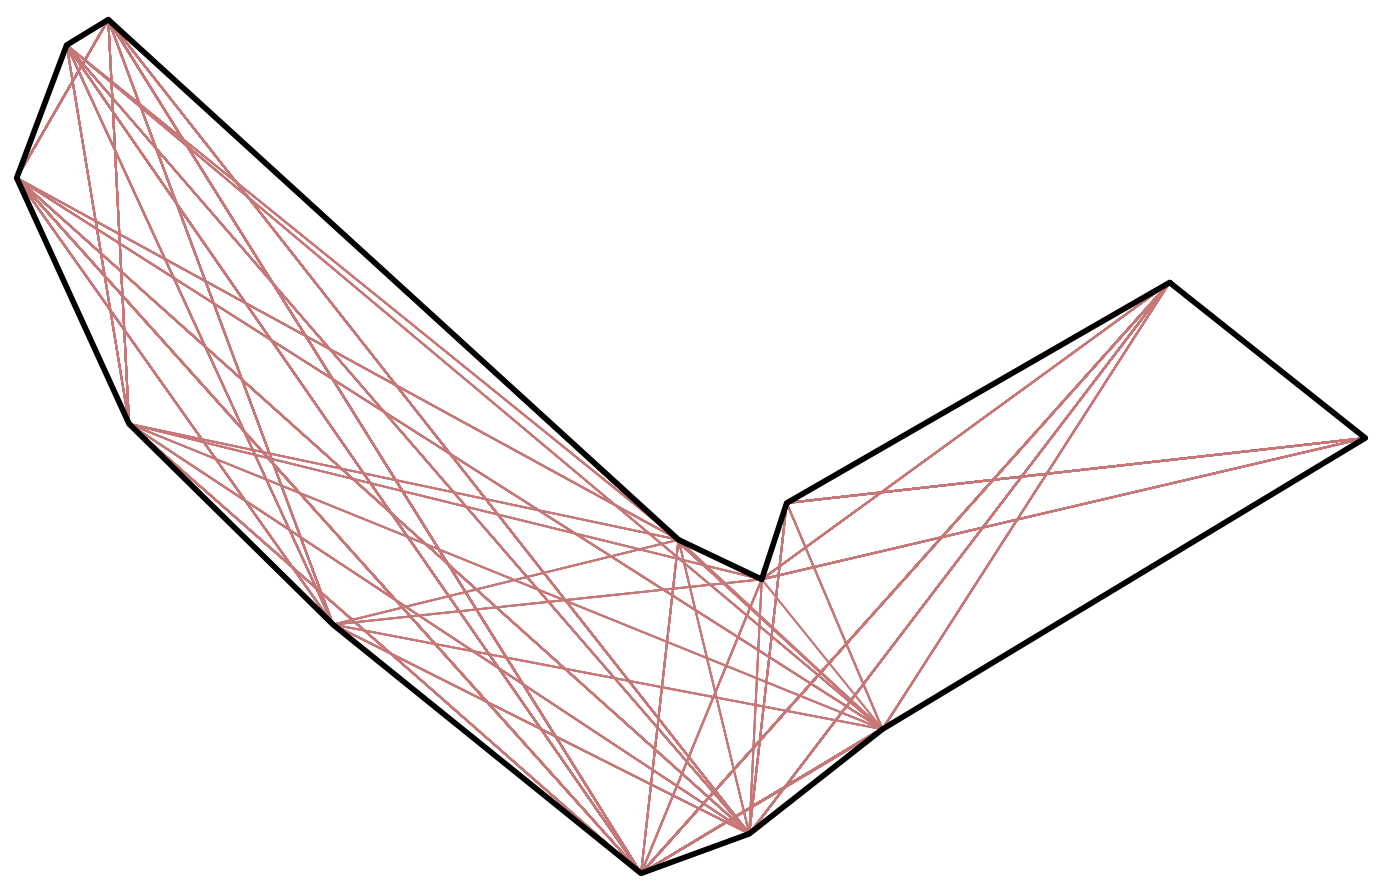
\includegraphics[width=0.8\textwidth]{images/routing/visibilityGraph.png}
	\caption{Visibility Graph in einer Flugzone}
	\label{fig:visibility-graph}
\end{figure}
Unschwer zu erkennen ist, dass deutlich weniger Flugrouten entlang von Polygon Kanten verlaufen. Dies ist ein deutlicher Fortschritt gegenüber dem ersten Konzept. Leider muss aber ehrlicherweise gesagt werden, dass die innere Ecke des L-förmigen Polygons sicher angefolgen wird, da es die vermeindlich kürzeste Route in einem nächsten Schritt darstellen wird. Aus diesem Grund wurde von einer weiterverfolgung des Algorithmus abgesehen.
\\
\subsubsection{Drittes Konzept: Straight Skeleton}
Durch die Recherchen für die zweite Lösung, war für uns klar, dass deine ideale Lösung eine mittenbetonte Flugroute empfehlen sollte. Eine einfach Lösung ohne viel implementations Aufwand war bereits in der \GLS{CGAL} Bibliothek vorhanden. Um \GLS{CGAL} dem \GLS{OGC} Standart zugänglich zu machen, wurde die \GLS{SFCGAL} Bibliothek in PostGIS verwendet. Diese ermöglichte es ein Straight Skeleton zu berechnen. Das Ergebnis für ein einfaches Polygon sah wie folgt aus:
\begin{figure}[h]
	\centering
	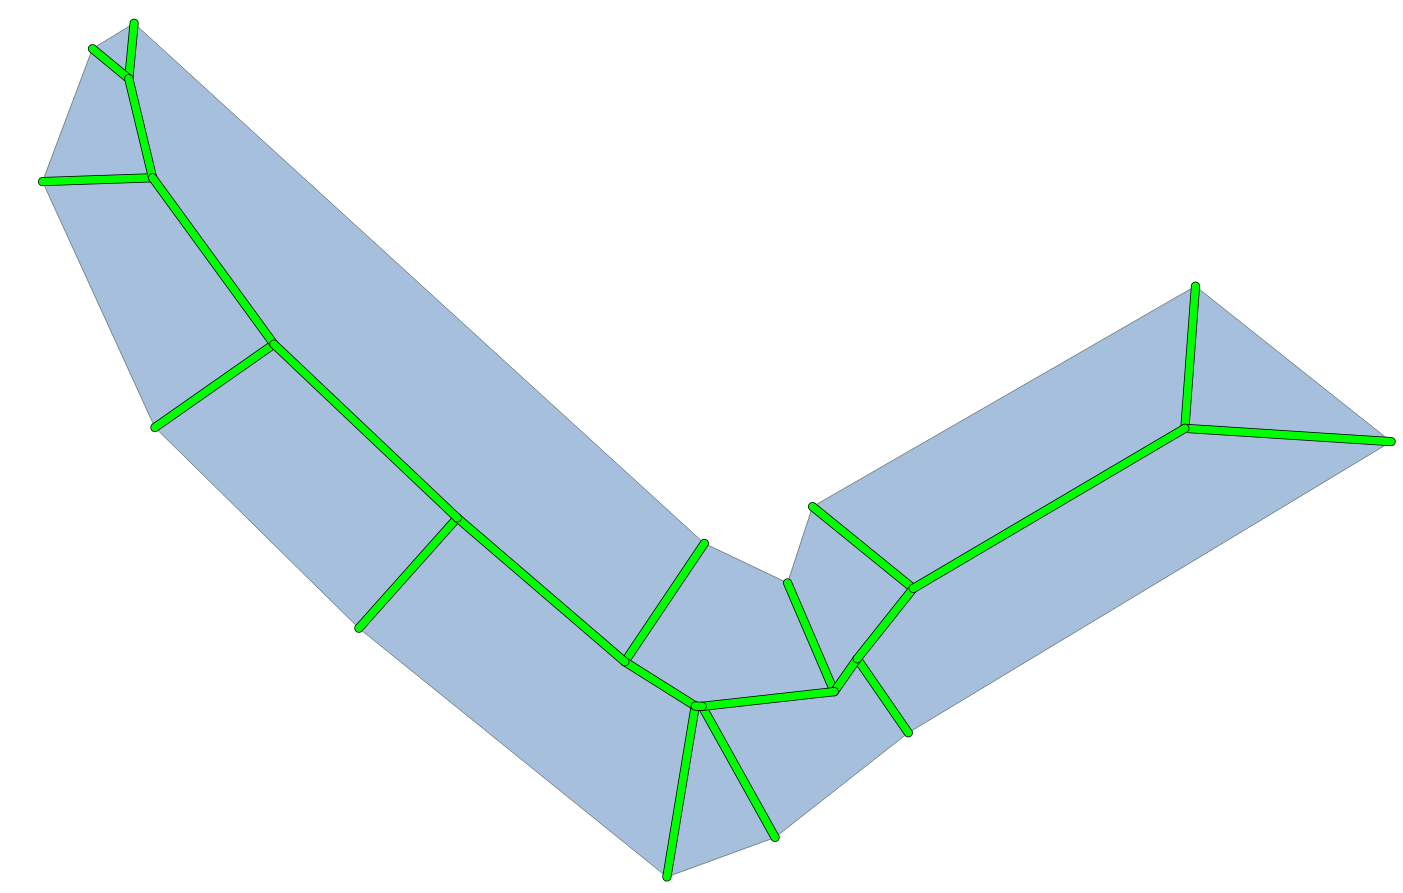
\includegraphics[width=0.8\textwidth]{images/routing/skeleton.png}
	\caption{Skeleton in Polygon}
	\label{fig:skeleton-in-polygon}
\end{figure}
Das Skeleton stellt quasi die Gipfel Linie eines Gebierges mit der Form des Polygons dar. Die Linie ist hier neon-grün eingezeichnet, um vollständigkeitshalber anzudeuten, dass sie bereits Teil einer fertigen Lösung ist. Von Hier ausgehend, fehlen nur noch die kürzesten Linien auf die Skeletonlinie. Diese sind bekanntlich die 2 Senkrechen von den Start und den Endpunkten auf die bestehende Linie.

\subsection{Graph Routing Algorithmus}
Nach der Herleitung des Graphen aus der Polygonstrukut, musste nun der passende Algorithmus gefunden werden um eine Lösung von A nach B zu finden. Es kamen 4 standart Algorithmen in Frage, wobei eine Algorithmus sich als besonders geeignet herausstellte.
\begin{itemize}
	\item{\textbf{BFS:} (\textit{Breadth-first search}) Die Breitensuche durchsucht einen Baum in der Breite. Sie ist unanfällig auf Zyklen im Baum und wäre ein guter Kandidat. Sie bringt garantiert eine Lösung, wenn eine Lösung vorhanden ist. Es muss aber nicht die 'optimale Lösung' (kürzester Pfad) sein, es wird der Pfad mit den wenigsten Knoten sein. \cite{AiClass}}
	\item{\textbf{DFS:} (\textit{Depth-first search}) Die Tiefensuche fängt an einem Knoten an und geht dann in die Tiefe. Das Problem ist, dass sie sehr anfällig auf Zyklen ist und dann ohne weiter Hilfsmittel (loop detection, pruning) nicht terminieren kann. Aus diesen Gründen ist diese Lösung nicht die Beste für unser Problem. \cite{AiClass}}
	\item{\textbf{A-Star:} Der A-Star Algorithmus arbeitet mit einer Heuristik und funktioniert dann effizienter wie die zwei bereits genannten Algorithmen. In unserem Fall war der A-Star Algorithmus zwar eine interessante Option, aber da wir uns am Anfang nicht auf die 'optimale Lösung' gestürzt haben, sondern eine 'garantierte Lösung' wollten, war die Heuristik und der damit verbunden Aufwand, ein Kriterium dagegen. \cite{AiClass}}
	\item{\textbf{Dijkstra:} Der Dijkstra-Algorithmus ist ebenfals ein klassischer Graphpropagierungsalgorithmus. Der Vorteil an ihm ist, dass er grundsätzlich ohne Heuristik auskommt und Robust mit Zyklen umgehen kann. Als Metrik kann in unserem Fall einfach eine Konstante genommen werden, so optimiert er auf die kleinste Anzahl Knotentraversierungen im Lösungspfad.}
\end{itemize}
Nach genauerem Betrachten der Algorithmen haben wir uns für den Dijkstra Algorithmus entschieden. Er liefert ohne Metrik eine ähnliche Lösung wie die BFS-Suche. Der Vorteil aber ist, dass der Umgang mit einer Metrik bereits konzepiert ist, was ihn deutlich von der klassischen BFS-Suche unterscheidet.
In einer ersten Version haben wir auf die Längen-Metrik verzichtet, das Ziel war eine Lösung zu finden ohne zu Garantieren, dass es sich hierbei um die beste handelt.

\subsection{Höhenhandling}
Bis anhin konnte angenommen werden, dass sämtliche Polygone der drei Zonentypen zusammengefasst werden können. Dieses aufsummierte Polygon war die Basis für die Routeberechnung. \\
Das Höhenhandling bildet nun der abschliessenden Schritt für die Routeberechung und benötigt wieder Informationen der einzelnen Polygone. Da die Höhe pro Zone individuell definiert werden kann. Dies geschieht in 2 Schritten.
\begin{itemize}
	\item{\textbf{Bestimmen der Zugehörigkeit:} In einem ersten Schritt werden die Zonen nach Höhe absteigend sortiert. Im Anschluss werden die differenzen von Polygonen entfernt, somit sind können die höher liegenden Polygone die Tieferliegenden abdecken. Dieses Abdecken, garantiert später, dass die Punkte nur einmal zugeordnet werden.}
	\item{\textbf{Setzten der Höhe:} Es wird über alle Punkte iteriert, und die höhe entsprechend dem Polygon indem es sich befindet gesetzt. Da die Überschneidungen nach Höhe im ersten Teil bereits vollzogen wurde, ist das Resultat eindeutig.}
\end{itemize}
\begin{figure}[h]
	\centering
	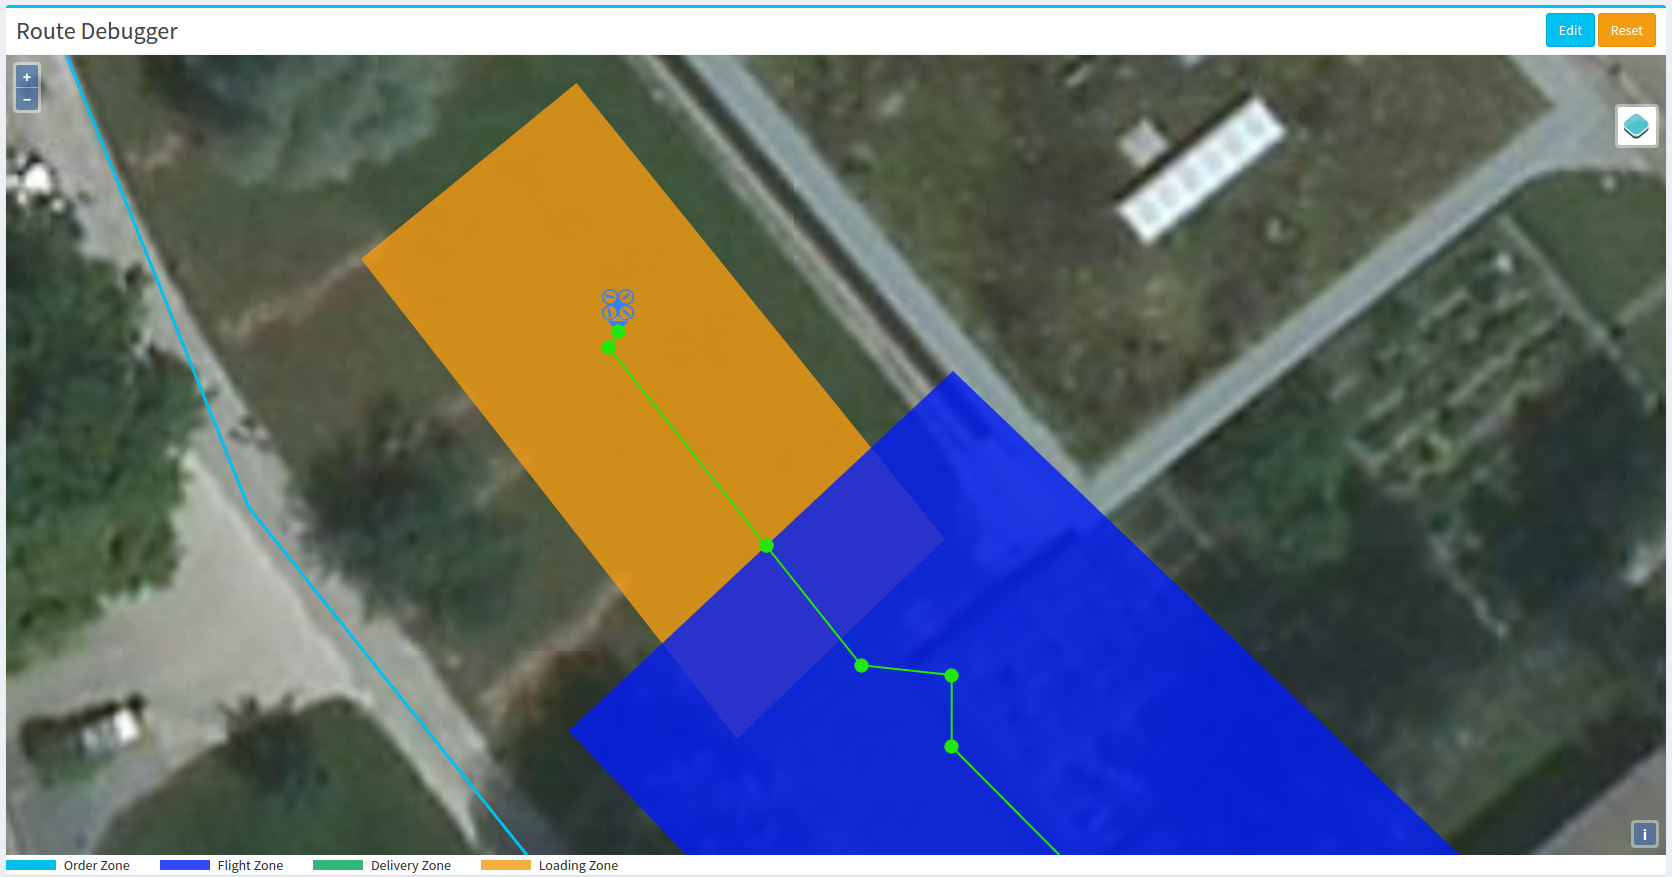
\includegraphics[width=1.0\textwidth]{images/routing/height_example.png}
	\caption{Beispiel der Höhe am Übergang zweier Polygone}
	\label{fig:polygon-border-example}
\end{figure}
Wie gemäss der Abbildung ersichtlich, ist trotz des langen geraden Pfades zwischen den zwei Zonen ein Punkt eingefügt. Im Grunde sind es zwei Punkte, die für den Wechsel der Flughöhe verantwortlich sind.
\newpage
\subsection{Wahl der Rückroute}
Das Bilden der Rückroute erfolgt in einem sehr einfachen verfahren. Bei der aktuellen Lösung werden Start und Endpunkt mit der dazugehörigen Aktion versehen. Im Falle des Endpunktes ist es in unserem Fall der Abwurf.
\\
Nun kann dieser Pfad genommen werden und umgedreht angehängt werden, wobei der letzte Punkt entfernt wird. Der letzte Punkt kommt nur einmal im Pfad vor, da dannach der nächste Punkt wieder der vorletzte sein soll. So ist garantiert, dass die Drohne den gleichen Rückweg wie hinweg verwendet um die Mission zu erfüllen. Diese Liste wird nun an den Autopiloten übergeben.
